\documentclass[journal]{IEEEtran}
\usepackage{cite}
\usepackage{amsmath,amssymb}
\usepackage{graphicx}
\usepackage{booktabs,array,multirow,tabularx}
\usepackage{algorithm}
\usepackage[noend]{algpseudocode}
\usepackage{tikz}
\usetikzlibrary{positioning,arrows.meta}
\usepackage{url}
\newcolumntype{Y}{>{\raggedright\arraybackslash}X}
\hyphenation{Light-GBM XG-Boost}

\begin{document}

\input{s00_front }
% ===== s01_introduction =====
\section{Introduction}
\IEEEPARstart{T}{he} rapid growth of Internet of Things (IoT) deployments has enlarged the attack surface available to botnet operators. Default credentials, unpatched firmware, and exposed management services allowed Mirai to assemble large denial-of-service botnets \cite{antonakakis2017}, and recent honeypot measurements show that the same credential-guessing and command patterns persist a decade later \cite{banoth2026}. Evasion is also evolving: routing-level malware built from legitimate system commands escaped most antivirus engines in a recent proof of concept \cite{abujazoh2025}. Detection therefore has to rely on behaviour rather than signatures.

Learning-based detectors have reported very high accuracy on benchmark data, using graph and temporal models \cite{babenko2026,chai2026}, radial basis function networks \cite{awad2026}, privacy-aware split learning \cite{aljaafreh2026}, and explainable feature selection \cite{georgiades2025,hua2026}. Three limitations recur. First, accurate models are frequently heavy, centralised, or opaque, which suits neither constrained IoT gateways nor analysts who must justify alerts. Second, evaluations often use class-balanced samples, random splits, or a single dataset, so results may not transfer to the heavily skewed traffic seen in practice. Third, lightweight models and feature reduction are rarely compared against strong tree ensembles under the same preprocessing, so the cost of simplification is not quantified.

\textbf{Research gap.} The literature reviewed in Phase 2 of this project shows no controlled comparison, on a large and heterogeneous IoT botnet corpus with natural class skew, of tree ensembles against a compact neural detector together with an explanation-guided feature reduction whose accuracy cost is measured.

\textbf{Contributions.} This work makes the following contributions.
\begin{itemize}
\item A reproducible benchmark on IoT-23 (binary botnet versus benign) of four standard classifiers and a 4,865-parameter compact MLP, with SMOTE and scaling confined to training data.
\item A SHAP-based global feature analysis of a random forest, identifying the traffic features that drive detection.
\item An ablation showing the effect of reducing the MLP to the three highest-ranked SHAP traffic features.
\item An explicit negative result: the compact MLP did not approach tree-ensemble performance, with a documented list of threats to validity and a fair comparison against base papers.
\end{itemize}

\textbf{Outline.} Section~II reviews related work, Section~III describes the methodology, Section~IV the experimental setup, Section~V the results, Section~VI the comparison with base papers, Section~VII the ablation, Section~VIII the discussion, and Section~IX concludes.
% ===== s02_related_work =====
\section{Related Work}
Table~\ref{tab:related} summarises the studies reviewed; they are discussed below by theme.

\textbf{Threat landscape.} Antonakakis et al.\ reconstructed Mirai's infection cycle and its reliance on default credentials \cite{antonakakis2017}. A two-week Cowrie and IoTPOT honeypot study found that \texttt{root} and \texttt{admin} dominate credential guesses, with Telnet receiving roughly fifteen times the top-source volume of SSH \cite{banoth2026}, but it proposes no detector and uses a single IP address. DCmal-2025 showed that routing commands can disconnect hosts while only 1.39\% to 9.72\% of about 72 antivirus engines flagged the executables \cite{abujazoh2025}, which motivates behaviour-based detection.

\textbf{Learning-based detection.} Power-consumption signatures have been classified with CNN, Transformer, and random forest models \cite{wakili2025}. A heterogeneous radial basis function network on 88 packet-length features of CTU-13 reported 97.86\% accuracy and a smooth degradation under Gaussian noise \cite{awad2026}. An AIoT architecture combining detection, honeypots, and sandboxing was validated in a virtual testbed \cite{memos2026}. These studies use one dataset or a controlled testbed.

\textbf{Graph and temporal models.} RIGS combines Rank Degree and PageRank-guided forest-fire sampling to train a GCN on large communication graphs, reducing time and memory but with only one or two positive test nodes per scenario \cite{chai2026}. A GNN--LSTM with temperature and Platt calibration reached 99.88\% accuracy on N-BaIoT but used class-balanced samples and random splits \cite{babenko2026}.

\textbf{Privacy-aware distributed learning.} Federated learning keeps raw traffic local for multi-stage botnet detection \cite{sudheera2026}. Traffic-constrained split learning with a six-block MLP achieved a mean macro-F1 of 98.27\% over three datasets at roughly one quarter of the federated communication cost \cite{aljaafreh2026}, but explanations and calibration were not studied.

\textbf{Explainability and feature selection.} SHAP, PDP, and ALE were used on MQTT and TCP features of an emulated ICU network, where SHAP-selected features matched the full feature set \cite{georgiades2025}. A comparison of SHAP, mutual information, ANOVA, and PCA on N-BaIoT reached 0.9994 accuracy with ten SHAP features and used a leave-one-device-out check, but did not measure computational cost \cite{hua2026}.

\textbf{Positioning.} The present work differs by evaluating a compact neural detector and tree baselines on IoT-23, whose natural class skew and multiple scenarios differ from the balanced benchmarks above, and by measuring what explanation-guided feature reduction costs.

\begin{table*}[!t]
\centering
\caption{Summary of key studies reviewed (values as reported by the original authors).}
\label{tab:related}
\scriptsize
\begin{tabularx}{\textwidth}{@{}l p{2.2cm} Y Y Y@{}}
\toprule
\textbf{Ref.} & \textbf{Theme} & \textbf{Data and method} & \textbf{Reported result} & \textbf{Key limitation} \\
\midrule
\cite{wakili2025} & Side-channel detection & IoT power traces; CNN, Transformer, RF & Power signatures separate botnet activity & Few device types; manipulated signatures untested \\
\cite{sudheera2026} & Federated detection & Simulated multi-stage botnet traffic; FL with data mining & Raw traffic stays on clients & Limited environment; poisoning untested \\
\cite{memos2026} & AIoT mitigation & Virtual AIoT testbed; ML, honeypots, sandbox & Feasible detection and response & Controlled testbed; overhead unknown \\
\cite{chai2026} & Graph sampling & CTU-13, NCC-2; RIGS with GCN & 40.9\,s and 3.26\,GB on NCC-2; accuracy 0.93--0.96 & 1--2 positive test nodes; static graphs \\
\cite{georgiades2025} & Explainable IDS & ICU-IoT; SHAP/PDP/ALE; six classifiers & Near-perfect KNN and RF with 13 features & One emulated dataset; explanations unmeasured \\
\cite{abujazoh2025} & Evasive malware & Proof-of-concept malware; VirusTotal & 1.39\%--9.72\% of engines detect & No detector; static analysis only \\
\cite{banoth2026} & Honeypot measurement & Cowrie and IoTPOT on one Azure VM, 2 weeks & \texttt{root} about 33\% (SSH), over 50\% (Telnet) & One IP address; no detection model \\
\cite{babenko2026} & Graph--temporal model & N-BaIoT, CICIoT2023; GNN--LSTM with calibration & 99.88\% accuracy, Brier 0.0015 (N-BaIoT) & Balanced sampling; random splits \\
\cite{aljaafreh2026} & Split learning & BoT-IoT, N-BaIoT, CIC-IDS2017; six-block MLP & Mean macro-F1 98.27\% & Archival data; no explanations \\
\cite{awad2026} & Robust RBF network & CTU-13; heterogeneous RBFNN & 97.86\% accuracy, AUC 0.9968 & One dataset; TCP only; noise not adversarial \\
\cite{hua2026} & SHAP feature selection & N-BaIoT; SHAP, MI, ANOVA, PCA; nine classifiers & LightGBM, top-10 SHAP: 0.9994 accuracy & Balanced classes; cost not measured \\
\bottomrule
\end{tabularx}
\end{table*}
% ===== s03_methodology =====
\section{Proposed Methodology}
\subsection{Problem Formulation}
Let $\mathcal{D}=\{(\mathbf{x}_i,y_i)\}_{i=1}^{n}$ be labelled connection records, where $\mathbf{x}_i\in\mathbb{R}^{d}$ is a numeric feature vector and $y_i\in\{0,1\}$ is the label ($1$ for any botnet-related activity, $0$ for benign). The goal is a classifier $f_{\theta}:\mathbb{R}^{d}\rightarrow[0,1]$ that maximises macro-F1 and ROC-AUC while keeping the false-positive rate and the per-sample cost low. A flow is flagged as an attack when $f_{\theta}(\mathbf{x})\ge 0.5$.

\subsection{Overall Pipeline}
Fig.~\ref{fig:arch} shows the implemented pipeline. Raw connection records are sampled, cleaned, encoded, split, balanced (training data only), and standardised before training. Four baselines and the compact MLP are evaluated on the same held-out test set, a SHAP analysis ranks features, and the highest-ranked traffic features define an ablation of the MLP.

\begin{figure*}[!t]
\centering
\resizebox{0.95\textwidth}{!}{%
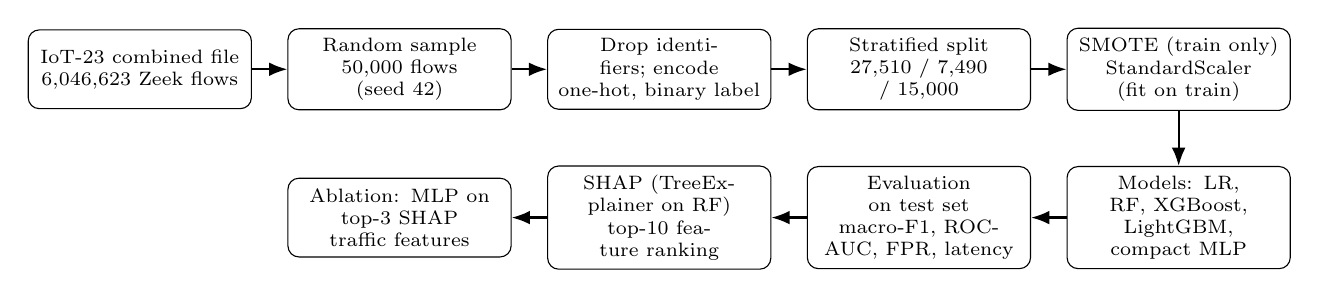
\begin{tikzpicture}[box/.style={draw, rounded corners, align=center, text width=2.6cm, minimum height=1.0cm, font=\scriptsize},
  arr/.style={-{Latex}, thick}]
\node[box] (n1) {IoT-23 combined file\\6,046,623 Zeek flows};
\node[box, right=0.45cm of n1] (n2) {Random sample\\50,000 flows (seed 42)};
\node[box, right=0.45cm of n2] (n3) {Drop identifiers; encode\\one-hot, binary label};
\node[box, right=0.45cm of n3] (n4) {Stratified split\\27,510 / 7,490 / 15,000};
\node[box, right=0.45cm of n4] (n5) {SMOTE (train only)\\StandardScaler (fit on train)};
\node[box, below=0.7cm of n5] (n6) {Models: LR, RF, XGBoost,\\LightGBM, compact MLP};
\node[box, left=0.45cm of n6] (n7) {Evaluation on test set\\macro-F1, ROC-AUC, FPR, latency};
\node[box, left=0.45cm of n7] (n8) {SHAP (TreeExplainer on RF)\\top-10 feature ranking};
\node[box, left=0.45cm of n8] (n9) {Ablation: MLP on\\top-3 SHAP traffic features};
\draw[arr] (n1)--(n2); \draw[arr] (n2)--(n3); \draw[arr] (n3)--(n4); \draw[arr] (n4)--(n5);
\draw[arr] (n5)--(n6); \draw[arr] (n6)--(n7); \draw[arr] (n7)--(n8); \draw[arr] (n8)--(n9);
\end{tikzpicture}}
\caption{Implemented experimental pipeline. Scaling and SMOTE use training data only.}
\label{fig:arch}
\end{figure*}

\subsection{Preprocessing and Class Balancing}
Spoofable identifiers (timestamp, connection identifier, source and destination address and port) are dropped so that a detector cannot rely on them. The Zeek placeholder \texttt{-} is converted to a missing value and then to zero. The categorical fields \texttt{proto}, \texttt{service}, \texttt{conn\_state}, and \texttt{history} are one-hot encoded, giving $d=42$ columns. SMOTE \cite{chawla2002} generates minority-class samples by interpolation,
\begin{equation}
\mathbf{x}_{\text{new}}=\mathbf{x}_i+\lambda(\mathbf{x}_{nn}-\mathbf{x}_i),\quad \lambda\sim\mathcal{U}(0,1),
\end{equation}
where $\mathbf{x}_{nn}$ is a nearest neighbour of $\mathbf{x}_i$ within the minority class. SMOTE is applied to the training partition only, and a \texttt{StandardScaler} fitted on the resulting training data standardises all partitions.

\subsection{Models}
\textbf{Baselines.} Logistic regression, random forest \cite{breiman2001}, XGBoost \cite{chen2016}, and LightGBM \cite{ke2017} are trained with the settings in Table~\ref{tab:hyper}.

\textbf{Compact MLP.} The compact detector has two hidden layers,
\begin{align}
\mathbf{h}_1&=\mathrm{ReLU}(\mathbf{W}_1\mathbf{x}+\mathbf{b}_1),\ \mathbf{W}_1\in\mathbb{R}^{64\times d},\\
\mathbf{h}_2&=\mathrm{ReLU}(\mathbf{W}_2\mathbf{h}_1+\mathbf{b}_2),\ \mathbf{W}_2\in\mathbb{R}^{32\times 64},\\
\hat{y}&=\sigma(\mathbf{w}_3^{\top}\mathbf{h}_2+b_3),
\end{align}
with dropout ($p=0.2$) after the first hidden layer during training. With $d=42$ it has 4,865 parameters, and with $d=3$ it has 2,369. It is trained by minimising the binary cross-entropy over a mini-batch of size $B$,
\begin{equation}
\mathcal{L}=-\frac{1}{B}\sum_{i=1}^{B}\big[y_i\log\hat{y}_i+(1-y_i)\log(1-\hat{y}_i)\big],
\end{equation}
using Adam \cite{kingma2015}.

\subsection{SHAP-Based Feature Ranking}
SHAP \cite{lundberg2017} assigns each feature $j$ a contribution $\phi_j(\mathbf{x})$ to a prediction. For tree models, TreeExplainer computes these values efficiently \cite{lundberg2020}. The global importance of feature $j$ over $n_s$ explained samples is
\begin{equation}
I_j=\frac{1}{n_s}\sum_{i=1}^{n_s}\left|\phi_j(\mathbf{x}_i)\right|,
\end{equation}
computed for the attack class of the random forest on $n_s=1{,}000$ flows. The three highest-ranked traffic features define the ablation in Section~VII.

\begin{algorithm}[!t]
\caption{Experimental procedure}
\label{alg:proc}
\begin{algorithmic}[1]
\Require Combined IoT-23 file, sample size $N=50{,}000$, seed $s=42$
\State Sample $N$ flows; drop identifiers; encode categoricals; set $y\leftarrow\mathbb{1}[\text{label}\neq\text{Benign}]$
\State Split stratified into $\mathcal{D}_{\text{train}},\mathcal{D}_{\text{val}},\mathcal{D}_{\text{test}}$
\State $\mathcal{D}_{\text{train}}\leftarrow\textsc{SMOTE}(\mathcal{D}_{\text{train}})$; fit scaler on $\mathcal{D}_{\text{train}}$; transform all partitions
\For{each baseline $m\in\{\text{LR},\text{RF},\text{XGB},\text{LGBM}\}$}
  \State Fit $m$ on $\mathcal{D}_{\text{train}}$; record metrics and inference time on $\mathcal{D}_{\text{test}}$
\EndFor
\State Train compact MLP for 20 epochs (Adam, BCE); record metrics
\State Compute $I_j$ with TreeExplainer on RF; select top-3 traffic features
\State Retrain the MLP on the top-3 features; record metrics
\end{algorithmic}
\end{algorithm}

\subsection{Changes Relative to the Phase 2 Plan}
The Phase 2 methodology proposed split or federated training, probability calibration, cross-dataset and device-disjoint evaluation, adversarial tests, and multi-seed statistical testing. The implemented work covers centralised training, SHAP feature ranking, and the ablation only. The remaining components were not implemented and are treated as future work (Section~IX).
\input{s04_experimental_setup }
\input{s05_results }
% ===== s06_comparison_base_papers =====
\section{Comparison with Base Papers}
The base papers are the studies whose methods this work builds on: SHAP-based feature selection \cite{georgiades2025,hua2026}, calibrated graph--temporal detection \cite{babenko2026}, and a compact MLP under split learning \cite{aljaafreh2026}.

\textbf{Summary.} Table~\ref{tab:related} lists their problem, data, method, results, and limitations.

\textbf{Quantitative comparison.} Table~\ref{tab:base} places our results next to the values reported by the base papers. Asterisks mark numbers copied from the original papers; none of their pipelines was re-implemented, and the datasets differ, so the table is not a like-for-like comparison.

\begin{table}[!t]
\centering
\caption{Reported results of base papers (*, from original papers) and this work (re-run on IoT-23).}
\label{tab:base}
\scriptsize
\begin{tabularx}{\columnwidth}{@{}l l Y@{}}
\toprule
\textbf{Study} & \textbf{Dataset} & \textbf{Best reported result} \\
\midrule
Georgiades \cite{georgiades2025}* & ICU-IoT (4 classes) & KNN, RF near-perfect precision, recall, accuracy \\
Babenko \cite{babenko2026}* & N-BaIoT & Accuracy 99.88\%, F1 0.9988, AUROC 0.9995 \\
Alja'afreh \cite{aljaafreh2026}* & BoT-IoT, N-BaIoT, CIC-IDS2017 & Mean macro-F1 98.27\% (split learning) \\
Hua \cite{hua2026}* & N-BaIoT (11 classes) & LightGBM, top-10 SHAP: accuracy 0.9994 \\
\textbf{This work, LightGBM} & IoT-23 (binary) & Macro-F1 0.9106, AUROC 0.9467, FPR 0.2526 \\
\textbf{This work, compact MLP} & IoT-23 (binary) & Macro-F1 0.6904, AUROC 0.7135, FPR 0.6115 \\
\bottomrule
\end{tabularx}
\end{table}

\textbf{Methodological comparison.} Like Hua et al.\ we rank features with SHAP and train gradient-boosted trees, and like Alja'afreh et al.\ we use a small MLP, but we train centrally, use IoT-23 with its natural skew in the test set, and add an ablation that measures the accuracy cost of reduction. We do not implement their split learning, calibration, or leave-one-device-out evaluation.

\textbf{Improvement analysis.} This work does not improve on the base papers. Our best macro-F1 (0.9106) is 0.0882 below the F1 of 0.9988* reported on N-BaIoT \cite{babenko2026} and 0.0721 below the 98.27\%* reported in \cite{aljaafreh2026}, and our compact MLP is far lower still. Because datasets, class balance, and splits differ, these gaps should not be read as a ranking of methods.

\textbf{Fairness and limitations.} The base papers use balanced or subsampled classes on N-BaIoT, BoT-IoT, or emulated data, whereas our test set retains an 11.5\% benign share and IoT-23 includes scanning, DDoS, and command-and-control scenarios. Our models are untuned, trained on 0.83\% of the file, and evaluated once. Factors that may explain the lower figures include dataset difficulty, no tuning, and the preprocessing choices, but this study did not isolate them.
% ===== s07_ablation =====
\section{Ablation Study}
The ablation replaces the 42 input columns of the compact MLP with the three highest-ranked genuine traffic features (\texttt{orig\_ip\_bytes}, \texttt{duration}, \texttt{orig\_pkts}) while keeping all other settings unchanged (Table~\ref{tab:abl}, Fig.~\ref{fig:abl}).

\begin{table}[!t]
\centering
\caption{Ablation of the compact MLP (single run, seed 42).}
\label{tab:abl}
\footnotesize
\begin{tabular}{@{}lccc@{}}
\toprule
\textbf{Metric} & \textbf{42 features} & \textbf{Top-3 features} & \textbf{Change} \\
\midrule
Parameters & 4,865 & 2,369 & $-51.3\%$ \\
Macro-F1 & 0.6904 & 0.6796 & $-0.0108$ \\
ROC-AUC & 0.7135 & 0.6401 & $-0.0734$ \\
FPR & 0.6115 & 0.6330 & $+0.0215$ \\
Final training loss & 0.4868 & 0.5218 & $+0.0350$ \\
\bottomrule
\end{tabular}
\end{table}

\begin{figure}[!t]
\centering
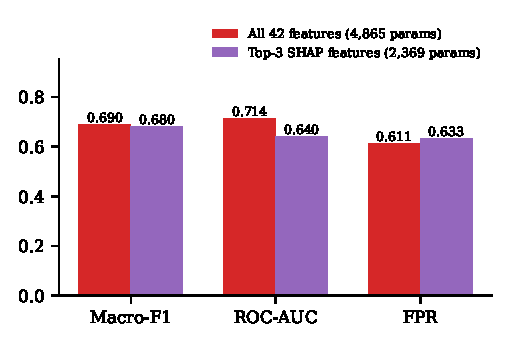
\includegraphics[width=0.85\columnwidth]{figures/fig_ablation.pdf}
\caption{Effect of reducing the compact MLP to the top-3 SHAP traffic features.}
\label{fig:abl}
\end{figure}

Reducing the input to three features cut the parameter count by 51.3\% but lowered ROC-AUC by 0.0734 and raised the FPR slightly, so the three features do not carry enough of the signal for this MLP. The macro-F1 change is small (0.0108) because both models already predict most flows as attacks. Other components (SMOTE, scaling, dropout, and the choice of explainer model) were not ablated, so their contributions are unknown.
% ===== s08_discussion =====
\section{Discussion}
\textbf{Why the results look as they do.} Tree ensembles handle heavy-tailed byte, packet, and duration counts and one-hot indicators without scaling, whereas the MLP was trained for only 20 epochs on standardised, SMOTE-balanced data and ended near the performance of logistic regression. These are hypotheses; the study did not test input transforms, longer training, or tuning.

\textbf{Practical implications.} For a skewed, heterogeneous corpus such as IoT-23, a gradient-boosted model offers the best accuracy among the tested options, while the compact MLP offers the lowest cost but not usable accuracy. Feature reduction guided by a random forest transferred poorly to the MLP.

\textbf{Strengths.} The pipeline keeps SMOTE and scaling inside the training partition, uses a test set with natural prevalence, reports macro-F1 and FPR rather than accuracy alone, and discloses its weaknesses.

\textbf{Limitations and failure cases.} The MLP and logistic regression flag about 61\% of benign flows, and every model has an FPR above 0.20. Failures by attack family were not analysed.

\textbf{Threats to validity.}
\begin{itemize}
\item \textit{Residual row index.} The unnamed leading column, apparently a saved row index, was kept as a feature and ranked fourth in SHAP importance. If rows in the source file are ordered by scenario or label, this column leaks label information to tree models and inflates their results relative to the MLP. The magnitude was not measured; the experiments should be repeated with this column removed.
\item \textit{Split design.} The split is random at flow level, so flows from the same capture or device can appear in training and test sets, and the proportions are 55/15/30 rather than 70/15/15.
\item \textit{Feature selection on test data.} SHAP importance was computed on a sample of the test set, so the ablation's feature choice is not independent of the test data.
\item \textit{Single run and sample.} One seed and a 50,000-flow sample were used, with no confidence intervals, tuning, or cross-validation.
\item \textit{Timing.} Inference times are single, coarse wall-clock measurements.
\end{itemize}

\textbf{Were the objectives met?} Partly. The study produced a lightweight and SHAP-explainable baseline and measured the cost of feature reduction. The Phase 2 objectives of privacy-aware training, calibrated probabilities, cross-dataset and device-disjoint generalisation, evasion testing, and statistical comparison were not achieved. The proposed compact MLP did not reach the accuracy of the tree baselines.
% ===== s09_conclusion =====
\section{Conclusion and Future Work}
On a 50,000-flow sample of IoT-23, LightGBM and XGBoost reached the highest ROC-AUC (0.9467) and LightGBM the highest macro-F1 (0.9106), whereas a 4,865-parameter MLP stayed at 0.6904 macro-F1 and 0.7135 ROC-AUC. SHAP highlighted flow volume and duration features, and reducing the MLP to the top three of them lowered ROC-AUC by 0.0734. The results are a transparent baseline and a negative finding for lightweight neural detection under this setup. Future work will remove the row-index column, use device-, scenario-, and time-disjoint splits, run multiple seeds with statistical tests, tune and transform inputs for the MLP, evaluate calibration and cross-dataset transfer, and add privacy-aware split or federated training.
% ===== s10_declarations =====
\section*{Declarations and Acknowledgements}

\noindent\textbf{Data and code availability.} IoT-23 is publicly available [13]. The implementation notebook (\texttt{phase3\_implementation.ipynb}), figure scripts, and \LaTeX{} source are hosted at \url{https://github.com/Humna-W-Janjua/IoT-Botnet-Detection_Computer-Networking}, with a backup copy of the notebook at \url{https://drive.google.com/file/d/1xAp6Vr9bSiu9G7Mb20ljF-S6xUJ2MPyq/view?usp=sharing}. Details on the combined CSV preparation are documented in the repository README.

\noindent\textbf{AI-tool usage declaration.} Generative AI assistance was used for debugging implementation code and refining manuscript language and formatting. All experiments, numerical results, and scientific claims were independently executed and verified by the authors.

\noindent\textbf{Conflict of interest.} The authors declare no conflict of interest.

\noindent\textbf{Funding.} This work received no external funding.



% ===== references =====
\begin{thebibliography}{99}
\bibitem{wakili2025} A. A. Wakili, S. Guni, S. A. Khan, W. Yu, and W. Jung, ``Advancing machine learning strategies for power consumption-based IoT botnet detection,'' \textit{Sensors}, vol. 25, p. 7553, 2025.
\bibitem{sudheera2026} K. L. K. Sudheera \textit{et al.}, ``Federated learning and data mining-based botnet attack detection framework for Internet of Things,'' \textit{Sensors}, vol. 26, p. 1573, 2026.
\bibitem{memos2026} V. A. Memos, C. L. Stergiou, A. I. Bermperis, A. P. Plageras, and K. E. Psannis, ``A novel architecture for mitigating botnet threats in AI-powered IoT environments,'' \textit{Sensors}, vol. 26, p. 572, 2026.
\bibitem{chai2026} J. Chai, Y. Shen, W. Tian, X. Sun, and L. Tian, ``RI graph sampling: A hybrid graph sampling method for large-scale botnet detection,'' \textit{Sensors}, vol. 26, p. 6154, 2026.
\bibitem{georgiades2025} M. Georgiades and F. Hussain, ``An explainable AI approach for interpretable cross-layer intrusion detection in Internet of Medical Things,'' \textit{Electronics}, vol. 14, p. 3218, 2025.
\bibitem{abujazoh2025} M. Abu-Jazoh, I. Almomani, and K. E. Sabri, ``DCmal-2025: A novel routing-based disconnectivity malware---development, impact, and countermeasures,'' \textit{Appl. Sci.}, vol. 15, p. 10219, 2025.
\bibitem{banoth2026} R. Banoth \textit{et al.}, ``Evolving IoT botnet threats and practical honeypot observation: A summary review and experimental study,'' \textit{J. Cybersecur. Priv.}, vol. 6, p. 82, 2026.
\bibitem{babenko2026} T. Babenko \textit{et al.}, ``Hybrid GNN--LSTM architecture for probabilistic IoT botnet detection with calibrated risk assessment,'' \textit{Computers}, vol. 15, p. 26, 2026.
\bibitem{aljaafreh2026} M. Alja'afreh, A. Karime, and A. Oukaira, ``Privacy-aware and resource-efficient split learning for IoT botnet detection: A multi-dataset experimental and systems evaluation,'' \textit{IoT}, vol. 7, p. 78, 2026.
\bibitem{awad2026} L. Awad, S. Al-Haj Baddar, and A. Sleit, ``Robust and noise-resilient botnet detection framework using heterogeneous radial basis function neural network,'' \textit{Appl. Sci.}, vol. 16, p. 3379, 2026.
\bibitem{hua2026} M. Hua, X. Zhang, and Y. Li, ``SHAP-guided feature selection for IoT botnet detection: A comparative study with conventional methods,'' \textit{Appl. Sci.}, vol. 16, p. 8840, 2026.
\bibitem{antonakakis2017} M. Antonakakis \textit{et al.}, ``Understanding the Mirai botnet,'' in \textit{Proc. 26th USENIX Security Symp.}, 2017, pp. 1093--1110.
\bibitem{iot23} S. Garcia, A. Parmisano, and M. J. Erquiaga, ``IoT-23: A labeled dataset with malicious and benign IoT network traffic,'' Zenodo, 2020, doi: 10.5281/zenodo.4743746.
\bibitem{chawla2002} N. V. Chawla, K. W. Bowyer, L. O. Hall, and W. P. Kegelmeyer, ``SMOTE: Synthetic minority over-sampling technique,'' \textit{J. Artif. Intell. Res.}, vol. 16, pp. 321--357, 2002.
\bibitem{breiman2001} L. Breiman, ``Random forests,'' \textit{Mach. Learn.}, vol. 45, no. 1, pp. 5--32, 2001.
\bibitem{chen2016} T. Chen and C. Guestrin, ``XGBoost: A scalable tree boosting system,'' in \textit{Proc. 22nd ACM SIGKDD}, 2016, pp. 785--794.
\bibitem{ke2017} G. Ke \textit{et al.}, ``LightGBM: A highly efficient gradient boosting decision tree,'' in \textit{Proc. NeurIPS}, vol. 30, 2017.
\bibitem{kingma2015} D. P. Kingma and J. Ba, ``Adam: A method for stochastic optimization,'' in \textit{Proc. ICLR}, 2015.
\bibitem{lundberg2017} S. M. Lundberg and S.-I. Lee, ``A unified approach to interpreting model predictions,'' in \textit{Proc. NeurIPS}, vol. 30, 2017, pp. 4765--4774.
\bibitem{lundberg2020} S. M. Lundberg \textit{et al.}, ``From local explanations to global understanding with explainable AI for trees,'' \textit{Nat. Mach. Intell.}, vol. 2, pp. 56--67, 2020.
\bibitem{pedregosa2011} F. Pedregosa \textit{et al.}, ``Scikit-learn: Machine learning in Python,'' \textit{J. Mach. Learn. Res.}, vol. 12, pp. 2825--2830, 2011.
\bibitem{lemaitre2017} G. Lema\^{i}tre, F. Nogueira, and C. K. Aridas, ``Imbalanced-learn: A Python toolbox to tackle the curse of imbalanced datasets in machine learning,'' \textit{J. Mach. Learn. Res.}, vol. 18, no. 17, pp. 1--5, 2017.
\bibitem{paszke2019} A. Paszke \textit{et al.}, ``PyTorch: An imperative style, high-performance deep learning library,'' in \textit{Proc. NeurIPS}, vol. 32, 2019.
\end{thebibliography}

\end{document}